


\subsection{Case Study 1: an Empirical Analysis of XOR Classification}
\label{sec:empirical}
First, we study the simplest linear-non-separable problem-- exclusive-or (XOR). Suppose that we have four two-dimensional input points $\mathbf{x}=[x_1,x_2]^T\in R^2$: $\{\mathbf{x}^1=[1,1]^T,\mathbf{x}^2=[0,0]^T\}\in C_+$ belongs to the positive class, while $\{\mathbf{x}^3=[1,0]^T,\mathbf{x}^4=[0,1]^T\}\in C_-$ the negative. 

As shown in Figure \ref{fig-xor}, we use a three-layer neural network to address the problem (left figure): $\mathbf{h_1}=\mathbf{x}+\mathbf{b}$ is a translation with  $\mathbf{b}=[b_1,b_2]^T\in R^2$ as the offset; $h_2=h_{1,1}*h_{1,2}$ is a non-linear layer, multiplying the first and second dimension of $\mathbf{h}_1$ and producing a scalar; $y$ is a linear classifier on $h_2$ parametrized by $w$. The original classification problem can be formulated as:
\begin{eqnarray*}
\arg\min_{w_1,\mathbf{b},w}\sum_{i=1}^4\log(1+\exp(-y^i*w*h^i_2))
%\label{eqn:final-cost}
\end{eqnarray*}

Suppose that we start from an initialization $\mathbf{b}=[0,0]^T$, all three samples $\{\mathbf{x}^2,\mathbf{x}^3,\mathbf{x}^4\}$ from different classes will produce the same representation $h_2=0$, which is not separable at all. It takes efforts to tune the learning rate to back-propagate $w,\mathbf{b}$ updates from the target $y$.

However, if we introduce the \textit{\textbf{uniform}} $L_2$ feature regularization as:
\begin{eqnarray*}
\arg\min_{w_1,\mathbf{b},w}\sum_{i=1}^4\log(1+\exp(-y^iwh^i_2))+\frac{\lambda_1}{2}||h^i_2||^2%+\lambda_2||w||^2
\end{eqnarray*}
Then, we have:
\begin{eqnarray}
\frac{\lambda_1}{2}\frac{\partial ||h_2||^2}{\partial\mathbf{b}}=\lambda_1
\binom{\mathbb{E}\{h_2(x_2+b_2)\}} {\mathbb{E}\{h_1(x_1+b_1)\}}
\label{eqn:xor-reg}
\end{eqnarray}
the gradient descent pulls Eqn(\ref{eqn:xor-reg}) towards zero, i.e., pulling $\mathbf{b}$ towards $b_1=-\mathbb{E}\{x_1\}=-0.5$ and $b_2=-\mathbb{E}\{x_2\}=-0.5$.
\begin{figure}
	\begin{center}
		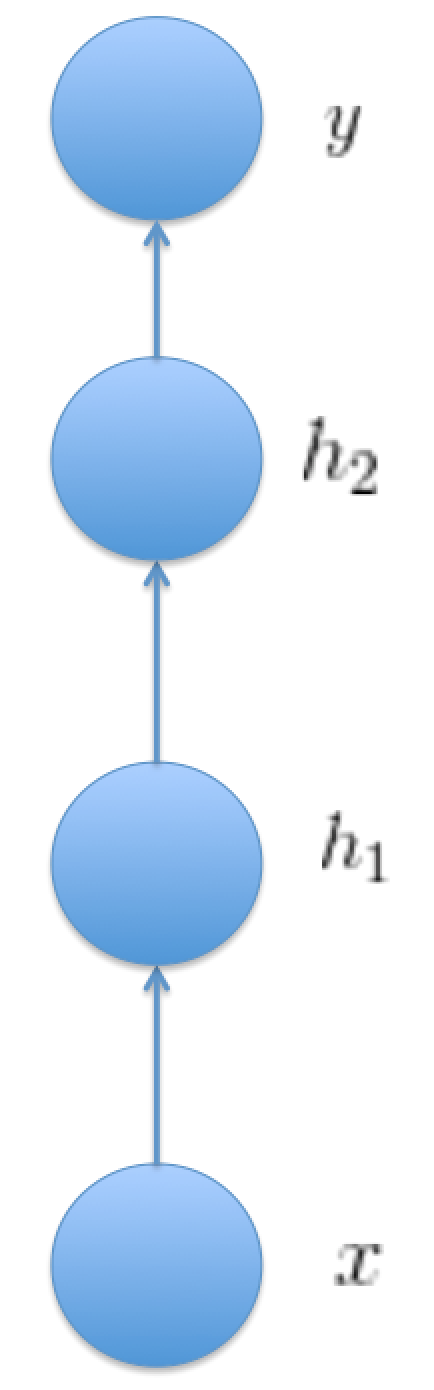
\includegraphics[width=0.1\columnwidth]{xor.png}
		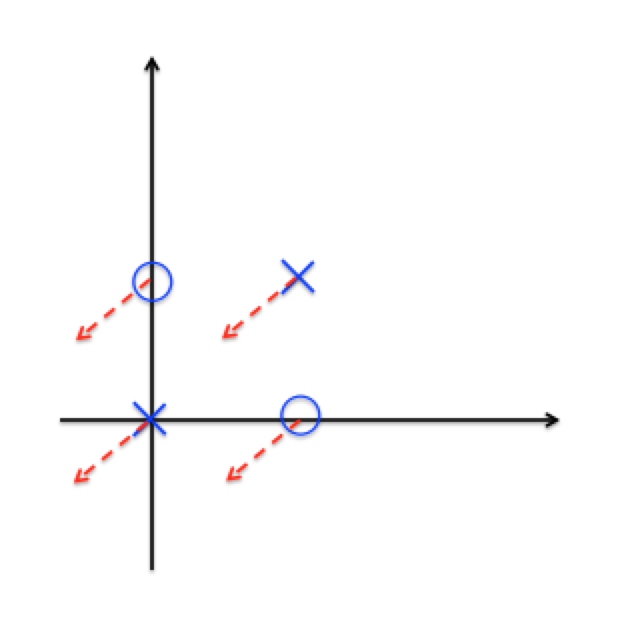
\includegraphics[width=0.35\columnwidth]{xor-analysis.png}
		%
		%	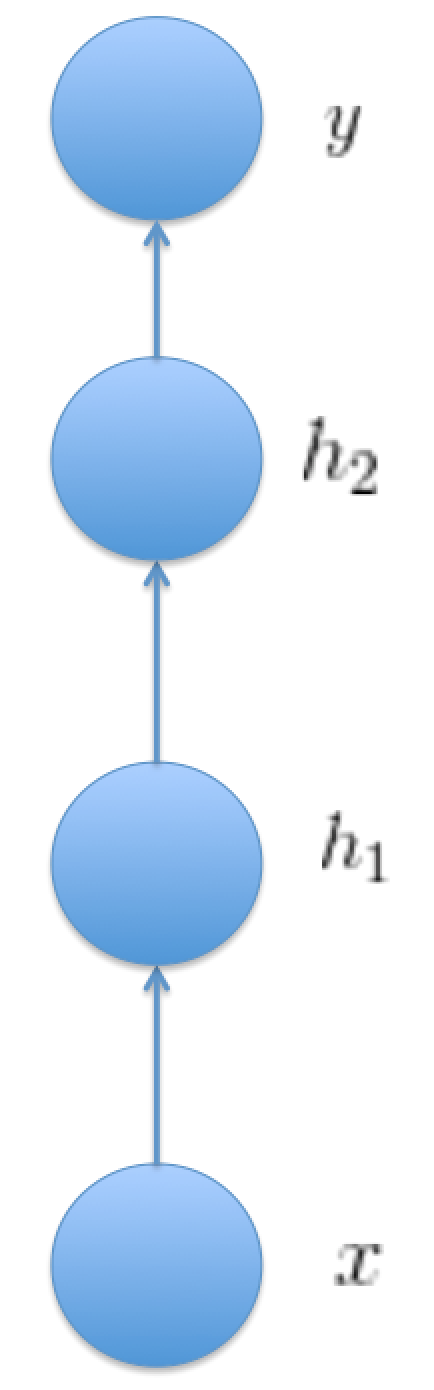
\includegraphics[width=0.3\columnwidth]{xor.png}\hspace{+0.5mm}
		%	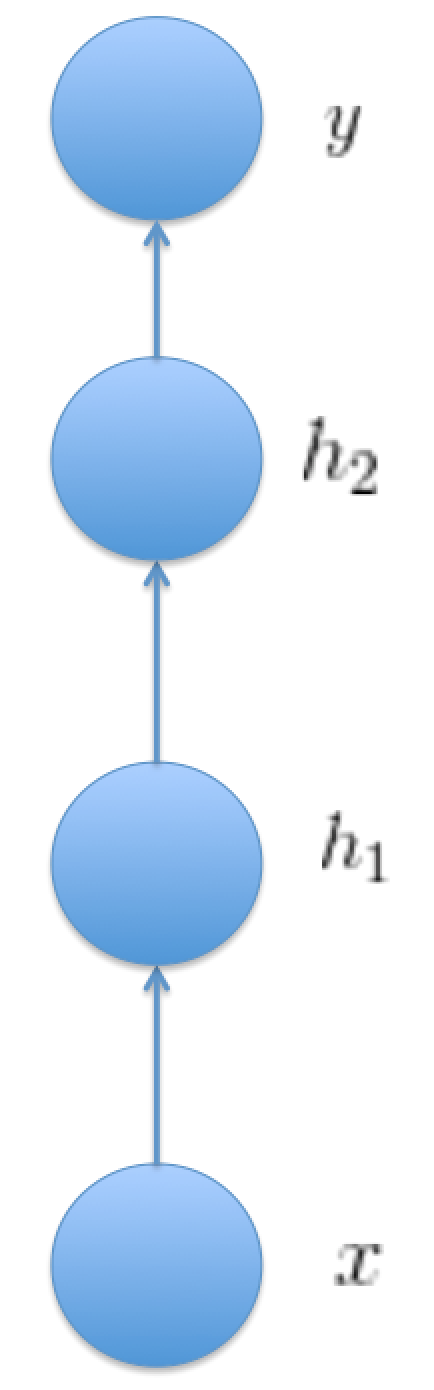
\includegraphics[width=0.3\columnwidth]{xor.png}\vspace{+1mm}\\
		%\end{center}
		%\hspace{+0mm}
		%\vspace{-2mm}
	\end{center}
	\caption{Case 1: an empirical study of the XOR classification task. {\bf The left figure:} the network structure we use: $h_1$ is a linear transformation, $h_2$ is a non-linear transform of $h_1$ and $y$ is the prediction; {\bf The right column:} The linear transformation maps $\mathbf{x}$ to $\mathbf{h_1}$. As shown in the red arrow, an $L_2$ norm penalty on $h_2$ centers the feature of $h_1$ and make the points from different sets separable. 'X's refer to positive examples, and 'O's are negative ones.}
	\label{fig-xor}
\end{figure}

%We can easily observe that the choice of $w,\mathbf{b}$ is critical to make the following feature $h_2$ trainable.  
As shown on the right of Figure \ref{fig-xor}, the gradient of feature regularization
pulls $\mathbf{h_1}$ along the direction of red arrows. Then, we have $h_2>0$ for positive examples and $h_2<0$ for negative ones, which means $h_2$ is linearly-separable. In summary, we can observe that:\\
\textbf{Empirically, the feature regularization \textit{centers} the representation $h_2=\phi(\mathbf{x})$ and makes the following classification more learnable}.\\
For the weighted case, the offset $\mathbf{b}$ have similar effects. It can be derived that when converged the feature representation will satisfy $\mathbb{E}\{\mathbf{h}_1\}=\mathbf{0}$ and $\mathbb{E}\{h_2\}$=0.
